\begin{figure*}[!tb]
\begin{center}
\begin{tikzpicture}
\node[inner sep=0pt] (a) at (0,0) {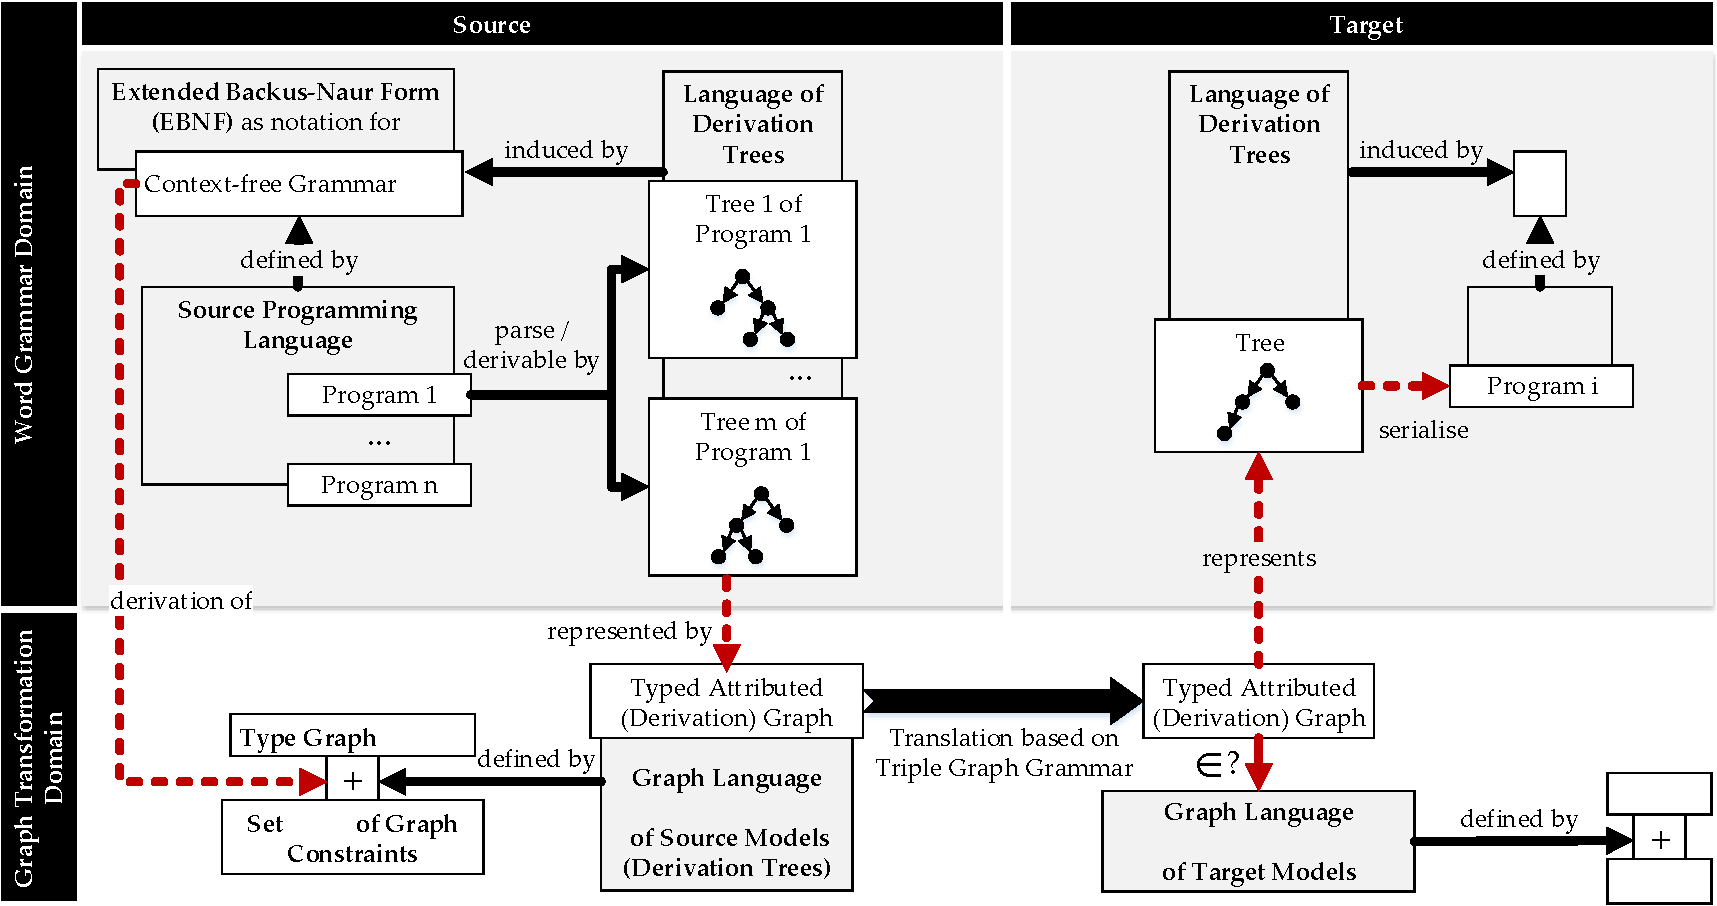
\includegraphics[width=\textwidth]{img/software_trans/software_trans.pdf}};
%\node[inner sep=0pt, right of=a,xshift=8.2cm] (b) {\includegraphics[width=.23\textwidth]{img/ast1.pdf}};
\node[inner sep=0pt] (b) at (-4.05,.95) {\scriptsize{$\Lang^S$}};
\node[inner sep=0pt] (c) at (5.85,1.1) {\scriptsize{$\Lang^T$}};
\node[inner sep=0pt] (d) at (-3.75,2.32) {\scriptsize{$G^S$}};
\node[inner sep=0pt] (e) at (5.85,2.3) {\scriptsize{$G^T$}};
\node[inner sep=0pt] (f) at (-3.7,-2.4) {\scriptsize{$\TG^S$}};
\node[inner sep=0pt] (g) at (-4.6,-3.15) {\scriptsize{$C^S$}};
\node[inner sep=0pt] (h) at (6.95,-2.92) {\scriptsize{$\TG^T$}};
\node[inner sep=0pt] (i) at (6.97,-3.67) {\scriptsize{$C^T$}};
\node[inner sep=0pt] (j) at (-1.1,-3.05) {\scriptsize{$\mathcal{VL}^S$}};
\node[inner sep=0pt] (k) at (3.5,-3.35) {\scriptsize{$\mathcal{VL}^T$}};
\end{tikzpicture}
\end{center}
\caption{Overview of Software Translations based on Triple Graph Grammars}
\label{fig:sec-compl-software-trans:softwaretrans}
\end{figure*}

\cref{fig:sec-compl-software-trans:softwaretrans} illustrates an overview of software translations based on triple graph grammars.
In software translations, programs written in a source programming language $\Lang^S$ are translated into programs (i.e. words) of a target (programming) language $\Lang^T$ (text-to-text translation) or into models of a target visual modelling language $\mathcal{VL}^T$ (text-to-model translation) (cf. \cref{fig:sec-compl-software-trans:software_trans_types}).
We assume that the source (target) word languages $\Lang^S$ ($\Lang^T$) are defined by context-free grammars $G^S$ ($G^T$) where the extended backus-naur form (EBNF) is used as a short-hand notation for context-free grammars in order to define programming languages.
Moreover, we assume that the target visual modelling language $\mathcal{VL}^T$ is a graph language of typed attributed graphs as models and is defined by an attributed type graph $\TG^T$ together with a set of graph constraints $C^T$.
Each context-free grammar induces a language of derivation trees that can be formed over the grammar.
Each derivation tree defines how a specific program (word) can be derived from the grammar.
Therefore, each derivation tree represents a specific program (word) of the language which is defined by the grammar.
Thus, the translation of programs is performed by translating their derivation trees.
In the following we give examples for an EBNF grammar, a derivation tree and the corresponding program which serve as running examples for the subsequent sections.

\begin{figure*}[!tb]
\begin{minipage}[c]{.51\textwidth}
\begin{lstlisting}
PROGRAM: first=CLASS
-----------------------------------------

CLASS  : 'class' name1=STRING (':' e=STR_LST)? '{' (attr1=ATTR)? '}' ('\n' (n1=CLASS | n2=ST))?
STR_LST: name2=STRING (',' n3=STR_LST)?
ATTR   : type=STRING name3=STRING ';' (n4=ATTR)?
-----------------------------------------

NEW    : 'new' cl2=STRING
ACCESS : obj=VAR '.' attr2=STRING
ST     : (a=ASG | p=PRINT | r=READ | i=IF | g=GOTO) ';' ('\n' n5=ST)?
ASG    : (a1=VAR | a2=ACCESS) '=' (a3=VAR | a4=ACCESS | a5=NEW)
PRINT  : 'print' out=ACCESS
READ   : 'read' (in1=VAR | in2=ACCESS)
IF     : 'if' c=COND 'then' body=ST 'end'
COND   : l=VAR ('='|'!=') (r1=STRING | r2=ACCESS | r3=NULL)
GOTO   : 'goto' line=INT
-----------------------------------------

terminal NULL   : 'null'
terminal STRING	: '"'.*'"'
terminal VAR    : ('a'..'z'|'A'..'Z')+
terminal INT    : (0..9)+
\end{lstlisting}
\end{minipage}
\begin{minipage}[c]{.45\textwidth}
\begin{lstlisting}
class "Person" { "String" "name"; "Person" "next"; }
class "Employee" : "Person" { "String" "salary"; }
-----------------------------------------
fst = new "Employee";
lst = fst;
read proceed;
-----------------------------------------
if proceed = "in" then
  read lst."name";
  read lst."salary";
  p = new "Employee";
  lst."next" = p;
  lst = p;
  goto 6;
end;
-----------------------------------------
if proceed = "out" then
  read name;
  current = fst;
  if name = current."name" then
    print current."salary";
  end;
  current = current."next";
  if current != null then
    goto 20;
  end;
  goto 6;
end;
\end{lstlisting}
\end{minipage}
\caption{Xtext EBNF Grammar of language \textit{Conditional-IN-OUT} (left) \& Program of language \textit{Conditional-IN-OUT} (right)}
\label{fig:sec-compl-software-trans:ebnf_xtext}
\end{figure*}

\begin{example}[Xtext EBNF Grammar]
\label{ex:sec-compl-software-trans:xtext_ebnf}
The EBNF grammar in \cref{fig:sec-compl-software-trans:ebnf_xtext} (left) is presented in Xtext notation and defines the ``toy'' programming language \textit{Conditional-IN-OUT}.
Xtext \cite{xtext} uses a special EBNF syntax for specifying context-free grammars of textual domain specific languages.
Xtext is widely used for the definition of programming languages and generates language parsers and editors automatically.

Each line represents a grammar rule.
In language \textit{Conditional-IN-OUT}, programs may \textsf{read} input from the user (line 14), assign it to a (member) variable (\textsf{ACCESS} (line 9)) \textsf{VAR} (line 22) and use the variable in comparisons with \textsf{STRING}s (line 21) and variables as conditions \textsf{COND} (line 16) in \textsf{if}-statements (line 15) in order to \textsf{print} some conditional output to the user (line 13).
Additionally to local variables \textsf{VAR}, data may also be stored in a more structured object-oriented way in member variables of classes.
Each \textsf{PROGRAM} \textsf{first} starts with a class definition (line 1).
Each \textsf{CLASS} (line 4) optionally refers (\textsf{n1}) to the next class or statement \textsf{ST} (\textsf{n2}).
Furthermore, each \textsf{CLASS} has a name (\textsf{name1}) of type \textsf{STRING} and optionally may inherit (reference \textsf{e}) from a set of classes that are given by a comma-separated list \textsf{STR\_LST} of \textsf{STRING}s (line 5) that are given after a colon \textsf{:} in the class definition and represent the class names.
Moreover, each \textsf{CLASS} may refer (\textsf{attr1}) to a set of attributes \textsf{ATTR} as member variables.
Each attribute (line 6) is given by a \textsf{type} and a name (\textsf{name3}), both defined by a \textsf{STRING}, and optionally may refer (\textsf{n4}) to the next attribute separated by a semicolon.
Object creation (line 9) is given by the keyword \textsf{new} followed by the class name (\textsf{cl2}) of the class from which the object is created.
\textsf{ACCESS} (line 10) to a member variable of an object is given by the standard dot-notation with a \textsf{VAR}iable that refers to the object (\textsf{obj}) on the left and the name of the member (\textsf{attr2}) on the right.
Statements \textsf{ST} (line 11) of a \textsf{PROGRAM} are assignments (\textsf{ASG}), \textsf{PRINT}, \textsf{READ}, \textsf{IF}-statements or \textsf{GOTO}s.
Furthermore, each statement \textsf{ST} optionally may refer (\textsf{n5}) to the next statement separated by a semicolon and newline.
Additionally to the statements that we already discussed above, assignments (line 12) are given by the symbol \textsf{=} with a (member) variable (\textsf{a2}) \textsf{a1} on the left and a (member) variable (\textsf{a4}) \textsf{a3} or object creation (\textsf{a5}) on the right.
Furthermore, \textsf{GOTO} statements (line 17) are given by the keyword \textsf{goto} together with the number \textsf{INT} of the \textsf{line} in which the execution of the program should proceed.

In Xtext notation, terminal symbols may be grouped in sorts and defined by so called terminal rules with regular expressions for each sort (lines 20-23).
Sort \textsf{STRING} (line 21) is defined by the regular expression \textsf{'"'.*'"'} allowing sequences of any character that are enclosed by quotation marks.
In contrast to \textsf{STRING}s, variables \textsf{VAR}s (line 22) are given by sequences of alphabetic characters that are not enclosed by quotation marks and \textsf{INT}s (line 23) are defined by sequences of numbers.
Moreover, the sort \textsf{NULL} (line 20) is given by the keyword \textsf{null} which refers to the null object.
\envEndMarker
\end{example}

\begin{example}[Program in language \textit{Conditional-IN-OUT}]
\label{ex:sec-compl-software-trans:prog}
In \cref{fig:sec-compl-software-trans:ebnf_xtext} (right), we present a program of language \textit{Conditional-IN-OUT} from \cref{ex:sec-compl-software-trans:xtext_ebnf}.
Two classes \textsf{Person} and \textsf{Employee} are defined.
\textsf{Person}s have a \textsf{name} and a \textsf{next} \textsf{Person} (line 1).
\textsf{Employees} are a special type of \textsf{Person}s by inheritance and additionally have a \textsf{salary} (line 2).
Lines 4-5 initialise an empty list of \textsf{Employee}s with a new \textsf{Employee} object as the first (\textsf{fst}) and last (\textsf{lst}) list element.
Line 6 reads the user input into variable \textsf{proceed}.
Depending on the user input, either the program asks the user to add a new \textsf{Employee} to the list (lines 8-15) or the program returns the \textsf{salary} of an existing \textsf{Employee} in the list (lines 17-27) where the \textsf{Employee} is identified by his \textsf{name}.
Finally, the program proceeds with line 6 or terminates if the user input differs from \textsf{``in''} or \textsf{``out''}.
\envEndMarker
\end{example}

\begin{figure*}[!tb]
\centering
\includegraphics[width=.47\textwidth]{img/software_trans/ast1.pdf}
\caption{Derivation Tree}
\label{fig:sec-compl-software-trans:ast}
\end{figure*}

\begin{example}[Derivation Tree]
\label{ex:sec-compl-software-trans:der_tree1}
The derivation tree of the program in \cref{ex:sec-compl-software-trans:prog} up to line 3 as induced by the grammar of \cref{ex:sec-compl-software-trans:xtext_ebnf} is presented in graphical notation in \cref{fig:sec-compl-software-trans:ast}.
Non-terminals become nodes in the tree, terminals of sorts \textsf{STRING},\textsf{VAR},\textsf{INT} and \textsf{NULL} become node attributes and references between grammar rules become edges.
Explicit keywords of the language (e.g. \textsf{class}) are not included in the tree.
By following the grammar, in derivation trees, the list of attributes of a class in a program are represented by edge \textsf{:attr1} pointing to the first attribute and edges \textsf{:n4} pointing to the next attribute.
Analogously, the lists of class definitions and the list of inherited classes for each class in a program are represented by edges \textsf{:first}, \textsf{:n1} and \textsf{:e}, \textsf{:n3}.
The complete tree that covers the whole program is given analogously.
\envEndMarker
\end{example}

Given a context-free grammar $G^S$ for source word language $\Lang^S$, then the translation of the induced derivation trees is specified by a triple graph grammar.
By \cref{fig:sec-compl-software-trans:softwaretrans}, each derivation tree is represented by a typed attributed graph in the source domain.
Then, the translation is performed by executing a model transformation on the graph based on the given triple graph grammar.
The result of the translation is a typed attributed graph in the target domain.
For text-to-model translations, the resulting graph is intended to directly serve as the resulting visual model in the target visual modelling language $\mathcal{VL}^T$ of the translation.
For text-to-text translations, the resulting graph is intended to be a representation of a derivation tree which is induced by the target context-free grammar $G^T$ of target word language $\Lang^T$.
The overall result of the text-to-text translation is obtained by flattening (serialising) the tree to a word (program) of the target language $\Lang^T$.
We demonstrate the graph-based approach for software translations by a translation of programs of language \textit{Conditional-IN-OUT} from \cref{ex:sec-compl-software-trans:xtext_ebnf} into UML class diagrams in \cref{ex:sec-compl-software-trans:trans}.
At first, we present the attributed type graphs of the source (\textit{Conditional-IN-OUT}) and target (class diagrams) domains of the translation in \cref{ex:sec-compl-software-trans:type_graphs}.

\begin{figure*}[!tb]
\centering
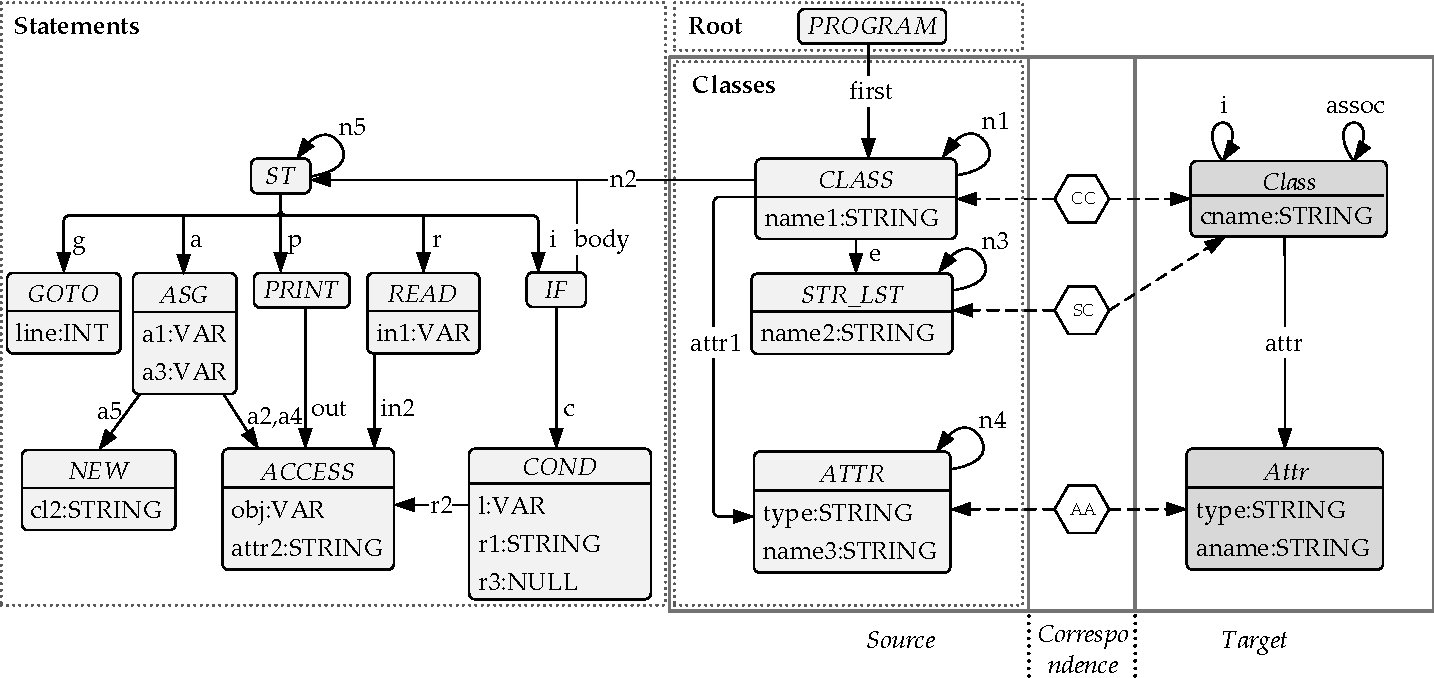
\includegraphics[width=.98\textwidth]{img/software_trans/tg.pdf}
\caption{EBNF Type Graph of Grammar \textit{Conditional-IN-OUT} (\textit{Root}+\textit{Statements}+\textit{Classes}) \& Triple Type Graph (\textit{Source} $\gets$ \textit{Correspondence} $\to$ \textit{Target})}
\label{fig:sec-compl-software-trans:tg_ebnf}
\end{figure*}

\begin{example}[Attributed Type Graphs]
\label{ex:sec-compl-software-trans:type_graphs}
\cref{fig:sec-compl-software-trans:tg_ebnf} illustrates both the attributed type graph of source language \textit{Conditional-IN-OUT} and the type graph of the target visual modelling language of UML class diagrams.
The type graph of \textit{Conditional-IN-OUT} is given by boxes \textit{Root},\textit{Statements} and \textit{Classes}.
The graph represents the structure of the \textit{Conditional-IN-OUT} grammar in \cref{fig:sec-compl-software-trans:ebnf_xtext} (left) where each grammar rule becomes a node in the graph and references between rules become edges or node attributes.
The type graph of class diagrams is given by box \textit{Target}.
Each diagram may have several \code{Class} nodes with a name (node attribute \code{cname}) of type \code{STRING} for each class.
Furthermore, each class may have several attributes (\code{Attr} nodes) each assigned by an \code{attr} edge.
Each attribute has a \code{type} and a name (node attribute \code{aname}) both of type \code{STRING}.
Moreover, there may be explicit inheritance relationships (\code{i} edges) and associations (\code{assoc} edges) between classes.
\envEndMarker
\end{example}

\begin{example}[Translation of \textit{Conditional-IN-OUT}]
\label{ex:sec-compl-software-trans:trans}
Each program of language \textit{Conditional-IN-OUT} from \cref{ex:sec-compl-software-trans:xtext_ebnf} is translated into an UML class diagram by transforming each class definition in the program into a \code{Class} node with optional attributes, association and inheritance relationships in the class diagram.
The translation of programs is performed by translating their derivation trees and specified by the triple graph grammar $\TGG=(\varnothing, P)$ with empty start graph $\varnothing$ and triple graph productions $P$ as given in \cref{fig:sec-compl-software-trans:rules}.
The triple graph production rules are typed over the triple type graph (\textit{Source} $\gets$ \textit{Correspondence} $\to$ \textit{Target}) in \cref{fig:sec-compl-software-trans:tg_ebnf}.
The triple type graph is given by boxes \textit{Classes} for \textit{Source} and \textit{Target} as described in \cref{ex:sec-compl-software-trans:type_graphs} together with a \textit{Correspondence} part which maps 
\begin{enumerate*}
\item \code{CLASS}es in programs to \code{Class} nodes in class diagrams (via correspondence nodes \code{CC}),
\item the names of inherited classes (\code{STR\_LST} nodes) to \code{Class} nodes (via \code{SC} correspondence nodes), and
\item class attributes (\code{ATTR} nodes) to class attributes (\code{Attr} nodes) (via \code{AA} correspondence nodes).
\end{enumerate*}
The production rules are presented in short-hand notation.
The elements of each triple rule are partitioned into the following three parts:
\begin{enumerate*}
\item source- (\textit{Conditional-IN-OUT}),
\item target-domain (UML class diagram) of the translation, and
\item correspondence part which maps elements from source to target and vice versa.
\end{enumerate*} 
For each rule $\LHS \to \RHS$ with left-hand side $\LHS$ and right-hand side $\RHS$, the $\LHS$ consists of all elements that are not marked with \textsf{++} whereas the $\RHS$ additionally consists of all elements that are marked with \textsf{++} and therefore, that are created when applying the rule to a $\LHS$ context.
Moreover, each rule is equipped with a negative application condition ($\NAC$) which restricts the rule application by describing a graph structure that is forbidden to exist for applying the rule.
For example, rule \textit{1:C2C} in \cref{fig:sec-compl-software-trans:rules} simultaneously creates a \textsf{CLASS} and a \textsf{Class} node with name \textsf{n} in the source and target domain with correspondence node \textsf{:CC} between both but only if the class diagram not already contains a \textsf{Class} node of the same name.
While the triple rules specify the translation, the translation itself is performed by applying operational forward translation rules that are derived from the triple rules.
Thus, from each rule $p \in P$, an operational forward translation rule $p_\FT$ is automatically derived.
For technical details we refer to Def. 7.29 in \cite{FAGT2} while the idea is rather straightforward.
Given a triple rule $p$, then the corresponding forward translation rule $p_\FT$ of $p$ translates those elements $E$ that are created by $p$ in the source domain into those elements $E'$ that are created by $p$ in the target domain together with the created correspondence part by adding elements $E'$ to elements $E$.
Moreover, the translation rule marks the translated elements as being translated in order to prevent a second translation of those elements.
In the following we give short descriptions for the forward translations rules of the triple rules in \cref{fig:sec-compl-software-trans:rules}.
The major challenges of the translation include:
\begin{enumerate*}
  \item the mapping of the list of class attributes for each class in a program to a star of attributes around the corresponding class node in the class diagram (rules \textit{2} \& \textit{3}),
  \item the mapping of the list of names of inherited classes for each class in a program to explicit inheritance relationships between actual class nodes in the class diagram (rules \textit{4} \& \textit{5}), and
  \item the mapping of implicit associations between classes in a program as given by the types of class attributes to explicit association relationships between actual class nodes in the class diagram (rules \textit{6} to \textit{10}).
\end{enumerate*}

\begin{figure*}[!tb]
\centering
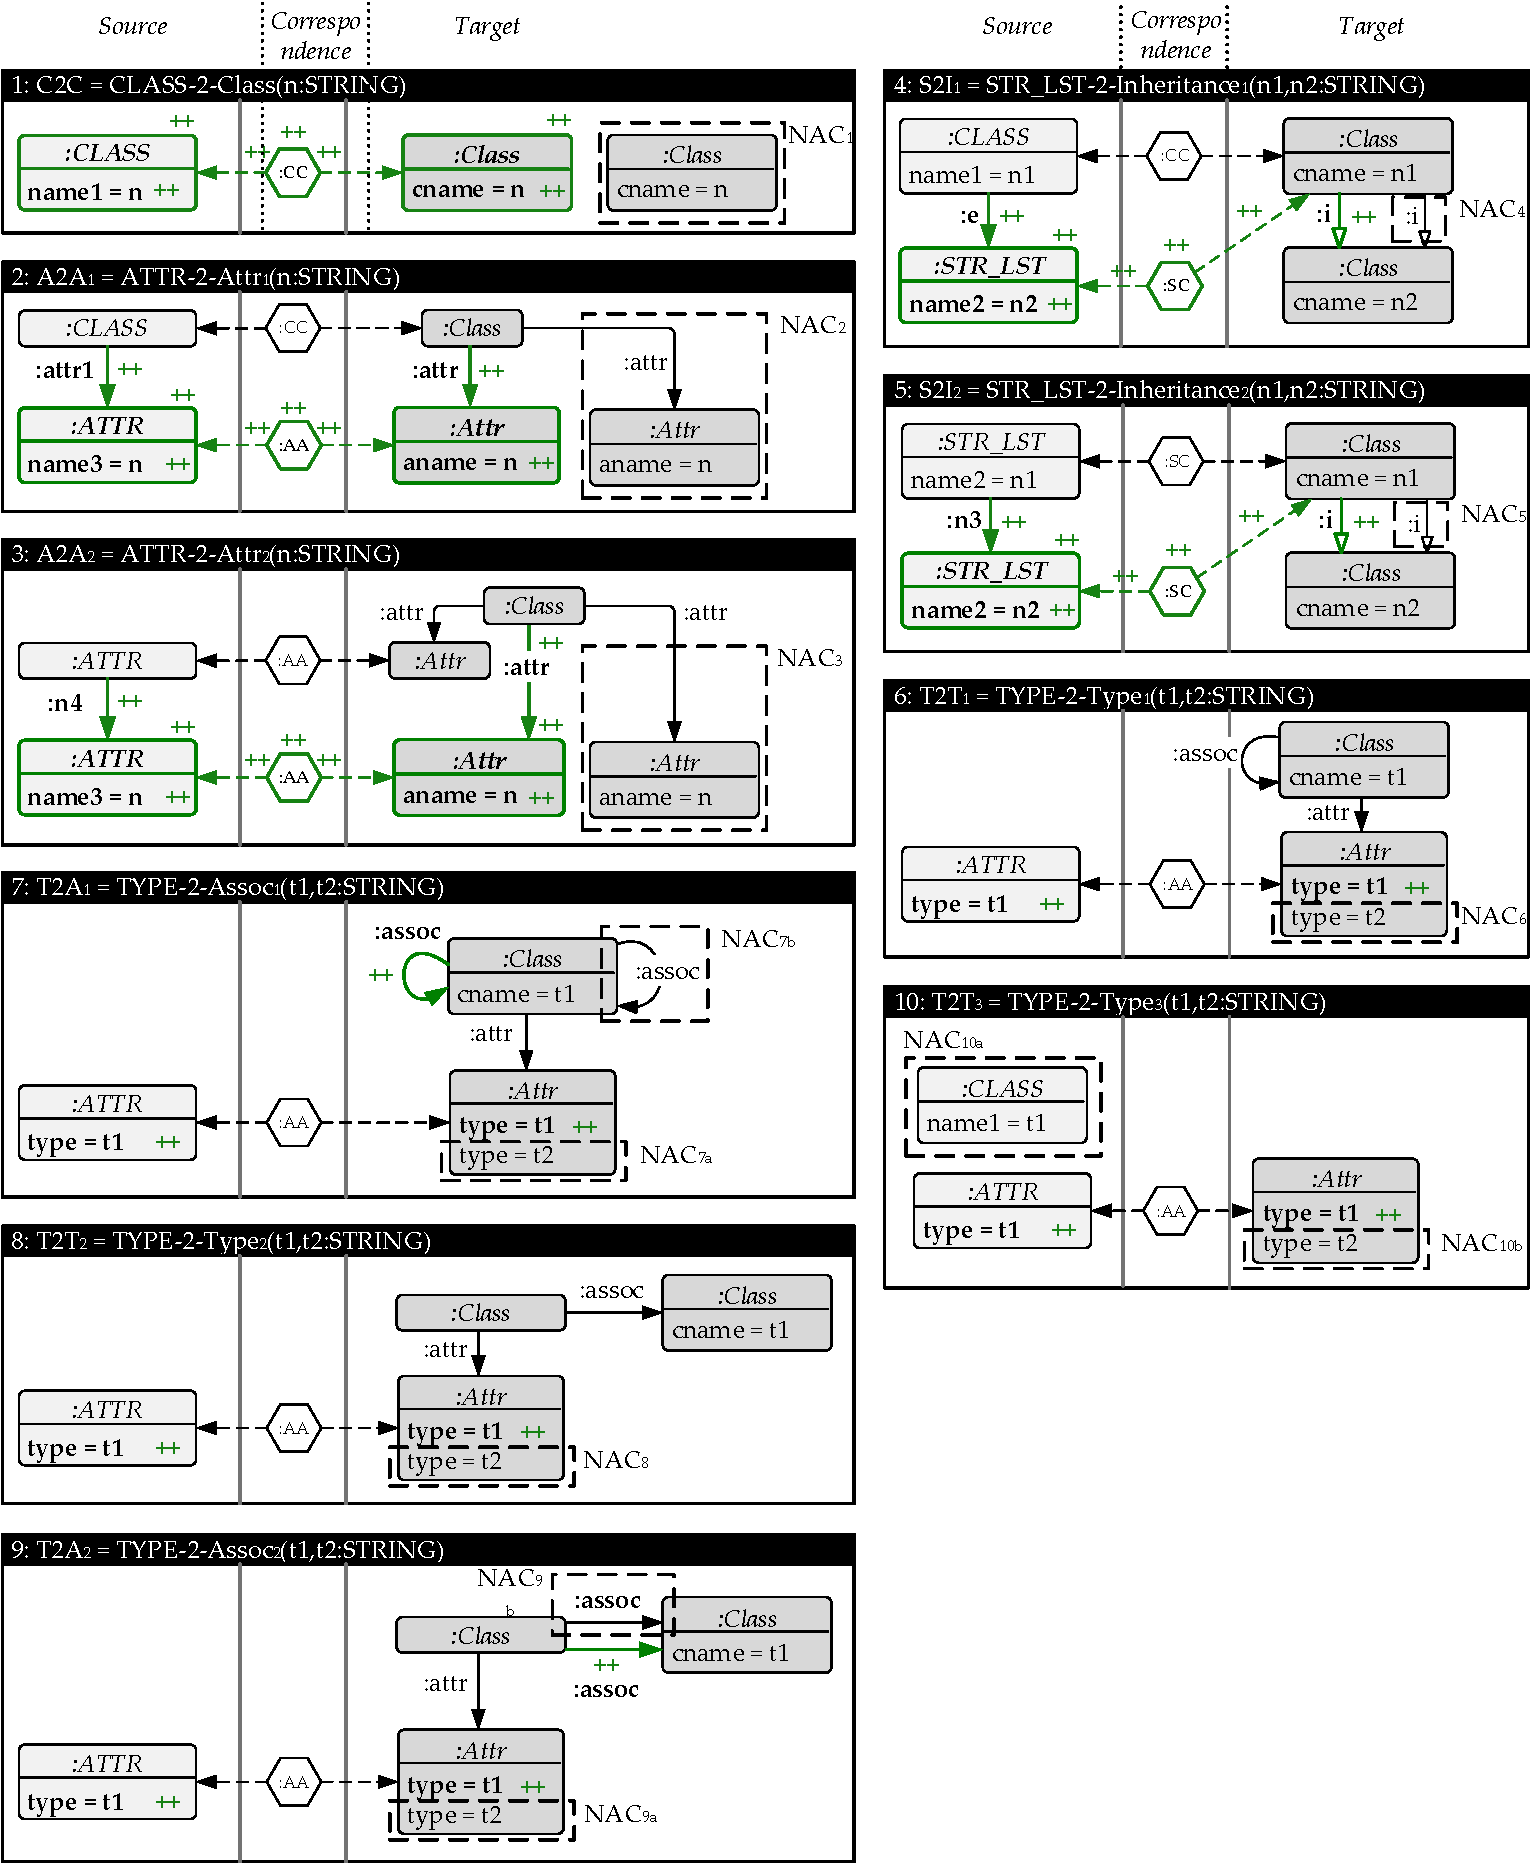
\includegraphics[width=\textwidth]{img/software_trans/rules.pdf}
\caption{Triple Graph Rules for Translation of Derivation Trees of Grammar \textit{Conditional-IN-OUT}}
\label{fig:sec-compl-software-trans:rules}
\end{figure*}

\begin{enumerate}
  \item Rule \textit{1:C2C}$_\FT$ translates a \textsf{CLASS} of name \textsf{n} in a program into a corresponding \textsf{Class} node with name \textsf{n} in the class diagram but only if there does not already exist a \textsf{Class} node with the same name (cf. $\NAC_1$).
  \item Rule \textit{2:A2A}$_{1,\FT}$ assumes that a \textsf{CLASS} in a program is already translated into a corresponding \textsf{Class} node in the class diagram.
  The rule translates the first class attribute (\textsf{:ATTR}) with name \textsf{n} of \textsf{:CLASS} into a corresponding attribute (\textsf{:Attr}) with name \textsf{n} of node \textsf{:Class} in the class diagram but only if node \textsf{:Class} does not already contain an attribute with the same name (cf. $\NAC_2$).
  \item Rule \textit{3:A2A}$_{2,\FT}$ translates the next attribute of the class into a corresponding attribute in the class diagram but analogously to rule \textit{2:A2A}$_{1,\FT}$, only if the correponding \textsf{Class} node in the diagram does not already contain an attribute with the same name (cf. $\NAC_3$).
  \item Rule \textit{4:S2I}$_{1,\FT}$ translates the name \textsf{n2} of the first inherited class for class \textsf{n1} in a program into an inheritance edge between the corresponding \textsf{Class} nodes in the class diagram but only if there does not already exist an inheritance edge between both nodes (cf. $\NAC_4$).
  \item Analogously to rule \textit{3:A2A}$_{2,\FT}$ for rule \textit{2:A2A}$_{1,\FT}$, rule \textit{5:S2I}$_{2,\FT}$ translates the name \textsf{n2} of the next inherited class for class \textsf{n1} into an inheritance edge between the corresponding \textsf{Class} nodes in the class diagram but only if there does not already exist an inheritance edge between both nodes (cf. $\NAC_5$).
  \item Rule \textit{10:T2T}$_{3,\FT}$ translates the type \textsf{t1} of a class attribute in a program into the same type of the corresponding attribute in the class diagram but only if type \textsf{t1} is not the name of a \textsf{CLASS} in the program and the attribute in the diagram does not already have a type \textsf{t2} (cf. $\NAC_{10a} \wedge \NAC_{10b}$).
  \item In contrast to rule \textit{10:T2T}$_{3,\FT}$, if type \textsf{t1} is the name of a \textsf{CLASS} in the program, then:
  \begin{enumerate}
    \item If \textsf{t1} is the name of the class of the class attribute and the corresponding \textsf{Class} node in the class diagram does already have a reflexive association (edge \textsf{:assoc}), then rule \textsf{6:T2T}$_1$ simply translates \textsf{t1} into the same type of the corresponding attribute in the class diagram but only if the attribute does not already have a type \textsf{t2} (cf. $\NAC_6$).
    \item If \textsf{t1} is the name of the class of the class attribute, then rule \textsf{7:T2A}$_1$ translates \textsf{t1} into the same type of the corresponding attribute together with a reflexive association for the corresponding \textsf{Class} node in the class diagram but only if the attribute does not already have a type \textsf{t2} and the \textsf{Class} node does not already have a reflexive association (cf. $\NAC_{7a} \wedge \NAC_{7b}$).
    \item If \textsf{t1} is not the name of the class of the class attribute but the name of another class in the program and there already exists an association between the corresponding \textsf{Class} nodes in the class diagram, then rule \textsf{8:T2T}$_2$ simply translates \textsf{t1} into the same type of the corresponding attribute in the class diagram but only if the attribute does not already have a type \textsf{t2} (cf. $\NAC_8$).
    \item If \textsf{t1} is not the name of the class of the class attribute but the name of another class in the program, then rule \textsf{9:T2A}$_2$ translates \textsf{t1} into the same type of the corresponding attribute together with an association between the corresponding \textsf{Class} nodes in the class diagram but only if the attribute does not already have a type \textsf{t2} and there does not already exist an association between the two \textsf{Class} nodes (cf. $\NAC_{9a} \wedge \NAC_{9b}$).
  \end{enumerate}
\end{enumerate}

\begin{figure*}[!tb]
\centering
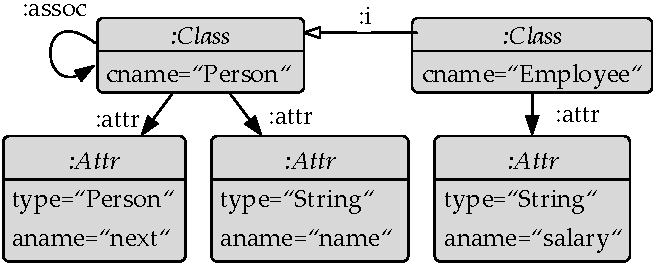
\includegraphics[width=.48\textwidth]{img/software_trans/result.pdf}
\caption{Result Graph}
\label{fig:sec-compl-software-trans:result}
\end{figure*}

The result of translating the derivation tree in \cref{ex:sec-compl-software-trans:der_tree1} by the forward translation rules from above is given by the typed attributed graph in \cref{fig:sec-compl-software-trans:result}.
The graph serves as a class diagram model in the target domain of the translation.
The list of attributes \textsf{name} and \textsf{next} of class \textsf{Person} becomes a star of attributes around the corresponding class node in the class diagram.
Furthermore, the implicit inheritance and association relationships between classes in the program become explicit edges in the class diagram.
\envEndMarker
\end{example}

\begin{remark}[Application Conditions in Translation]
The rules in \cref{ex:sec-compl-software-trans:trans} make extensive use of negative application conditions (NACs) in order to control the translation.
While the negative application conditions $\NAC_{7b},\NAC_{9b}$ and $\NAC_{10a}$ ensure that at most one rule of rules \textit{6} to \textit{10} as applicable to a given context at the same time, the other application conditions rather define restrictions of the target language of the translation, i.e., restrictions that need to be satisfied by each class diagram which results from a translation of a \textit{Conditional-IN-OUT} program.
\begin{enumerate*}
\item $\NAC_1$ ensures that each resulting class diagram does not contain two classes with the same name,
\item $\NAC_2$ and $\NAC_3$ ensure that each resulting class diagram does not contain a class with two or more class attributes having the same name,
\item $\NAC_4$ and $\NAC_5$ ensure that each resulting class diagram does contain at most one inheritance edge between each two classes,
\item $\NAC_6,\NAC_{7a},\NAC_8,\NAC_{9a}$ and $\NAC_{10b}$ ensure that each resulting class diagram does contain at most one type for each class attribute, and
\item $\NAC_{7b}$ and $\NAC_{9b}$ ensure that each resulting class diagram does contain at most one association between each two classes. \envEndMarker
\end{enumerate*}
\end{remark}